% Options for packages loaded elsewhere
\PassOptionsToPackage{unicode}{hyperref}
\PassOptionsToPackage{hyphens}{url}
%
\documentclass[
]{article}
\usepackage{lmodern}
\usepackage{amssymb,amsmath}
\usepackage{ifxetex,ifluatex}
\ifnum 0\ifxetex 1\fi\ifluatex 1\fi=0 % if pdftex
  \usepackage[T1]{fontenc}
  \usepackage[utf8]{inputenc}
  \usepackage{textcomp} % provide euro and other symbols
\else % if luatex or xetex
  \usepackage{unicode-math}
  \defaultfontfeatures{Scale=MatchLowercase}
  \defaultfontfeatures[\rmfamily]{Ligatures=TeX,Scale=1}
\fi
% Use upquote if available, for straight quotes in verbatim environments
\IfFileExists{upquote.sty}{\usepackage{upquote}}{}
\IfFileExists{microtype.sty}{% use microtype if available
  \usepackage[]{microtype}
  \UseMicrotypeSet[protrusion]{basicmath} % disable protrusion for tt fonts
}{}
\makeatletter
\@ifundefined{KOMAClassName}{% if non-KOMA class
  \IfFileExists{parskip.sty}{%
    \usepackage{parskip}
  }{% else
    \setlength{\parindent}{0pt}
    \setlength{\parskip}{6pt plus 2pt minus 1pt}}
}{% if KOMA class
  \KOMAoptions{parskip=half}}
\makeatother
\usepackage{xcolor}
\IfFileExists{xurl.sty}{\usepackage{xurl}}{} % add URL line breaks if available
\IfFileExists{bookmark.sty}{\usepackage{bookmark}}{\usepackage{hyperref}}
\hypersetup{
  pdftitle={Variações morfológicas em duas espécies de Serpentes},
  pdfauthor={Natalia Malaquias Souto},
  hidelinks,
  pdfcreator={LaTeX via pandoc}}
\urlstyle{same} % disable monospaced font for URLs
\usepackage[margin=1in]{geometry}
\usepackage{graphicx,grffile}
\makeatletter
\def\maxwidth{\ifdim\Gin@nat@width>\linewidth\linewidth\else\Gin@nat@width\fi}
\def\maxheight{\ifdim\Gin@nat@height>\textheight\textheight\else\Gin@nat@height\fi}
\makeatother
% Scale images if necessary, so that they will not overflow the page
% margins by default, and it is still possible to overwrite the defaults
% using explicit options in \includegraphics[width, height, ...]{}
\setkeys{Gin}{width=\maxwidth,height=\maxheight,keepaspectratio}
% Set default figure placement to htbp
\makeatletter
\def\fps@figure{htbp}
\makeatother
\setlength{\emergencystretch}{3em} % prevent overfull lines
\providecommand{\tightlist}{%
  \setlength{\itemsep}{0pt}\setlength{\parskip}{0pt}}
\setcounter{secnumdepth}{-\maxdimen} % remove section numbering

\title{Variações morfológicas em duas espécies de Serpentes}
\author{Natalia Malaquias Souto}
\date{24 de março de 2020}

\begin{document}
\maketitle

\hypertarget{introduuxe7uxe3o}{%
\subsection{Introdução}\label{introduuxe7uxe3o}}

A tribo Xenodontini é diagnosticada por características do hemipênis,
como presença de disco apical nu em cada lobo do hemipênis o qual não
apresenta capitação ou cálices (Myers, 1986; Jenner \& Dowling, 1985;
Zaher et al., 1999, 2009b). Dixon (1980) reconhece seis gêneros
pertencentes à tribo Xenodontini: \emph{Erythrolamprus} Boie, 1826;
\emph{Xenodon} Boie, 1826; \emph{Liophis} Wagler, 1830;
\emph{Lystrophis} Cope, 1885; \emph{Umbrivaga} Roze, 1964 e
\emph{Waglerophis} Romano \& Hoge, 1972. Neste estudo o autor examinou
uma quantidade significativa de espécimes e sinonimizou os gêneros
\emph{Dromicus} Bibron, 1843, \emph{Leimadophis} Fitzinger, 1843 e
\emph{Lygophis} Fitzinger, 1843 a \emph{Liophis}, com base na
complexidade das variações apresentadas pela maioria das espécies
pertencentes a esses quatro gêneros em relação a caracteres
osteológicos, merísticos e morfométricos.

Segundo Dixon (1980) é possível separar \emph{Liophis} dos demais
gêneros da tribo Xenodontini através das seguintes características:
possuir 10 ou mais dentes palatinos; ter osso maxilar e dentes
associados orientados verticalmente; osso prémaxilar com fraca conexão
com os ossos septomaxilar e nasais; osso maxilar longo e com pouca
mobilidade; processo maxilar do ectopterigoide sem uma margem central
profunda e projeções anterolaterais do osso frontal bem desenvolvidas.
Contudo, em análises com base em dados moleculares o gênero
\emph{Liophis} se mostra parafilético em relação a \emph{Erythrolamprus}
(Vidal et al., 2000, 2010; Zaher et al., 2009 e Grazziotin et al.,
2012).

Zaher et al.~(2009), com base em dados moleculares, sinonimizaram
\emph{Lystrophis} e \emph{Waglerophis} a \emph{Xenodon}, revalidaram
\emph{Lygophis} e sinonimizaram \emph{Erythrolamprus} a \emph{Liophis}.
Entretanto, Curcio et al.~(2009) não reconhecem as mudanças adotadas por
Zaher et al.~(2009) em relação a \emph{Lygophis} e \emph{Liophis},
argumentando que as mesmas são prematuras visto que um número maior de
táxons devem ser incluídos na análise, inclusive as espécies-tipo. Além
disso, chamam atenção para um erro de nomenclatura cometido, já que o
nome \emph{Erythrolamprus} tem prioridade sobre \emph{Liophis} por ter
sido descrito antes. Vidal et al.~(2010) corroboram os resultados
encontrados por Zaher et al.(2009) em relação aos gêneros
\emph{Lygophis} e \emph{Xenodon}, mas mantêm os gêneros
\emph{Erythrolamprus} e \emph{Liophis}, ressaltando o parafiletismo do
último e a necessidade de análises mais específicas sobre estes táxons.
Grazziotin et al.~(2012), após incluir novos táxons às análises,
sinonimizam \emph{Liophis} a \emph{Erythrolamprus} (as espécies-tipo dos
gêneros não foram incluídas na análise), porém afirmam que essa
conformação provavelmente será modificada por análises futuras com uma
amostragem mais representativa. Wallach et al.~(2014) reconhecem os
gêneros \emph{Liophis}, \emph{Lygophis} e \emph{Erythrolamprus}. No
presente estudo adotamos a postura mais conservadora de Curcio \emph{et
al.} (2009), Vidal \emph{et al.} (2010) e Wallach \emph{et al.} (2014)
reconhecendo o gênero Liophis. Liophis (\emph{sensu} Dixon, 1980) possui
mais de 40 espécies válidas (Curcio et al., 2009), sendo que oito delas
estão atualmente alocadas no gênero \emph{Lygophis} (Zaher et al.,
2009b). O gênero \emph{Liophis} encontra-se distribuído ao longo da
América do Sul e parte da América central, inclusive em ilhas do Caribe
(Dixon, 1980; 1989; 2000). As relações interespecíficas dentro do gênero
não estão completamente esclarecidas e ainda existem muitos problemas na
taxonomia alfa de diversas espécies o que dificulta a determinação do
relacionamento entre as espécies (Dixon, 1983a; 1983b; Fernandes et al.,
2002)

\hypertarget{histuxf3rico-taxonuxf4mico}{%
\subsubsection{Histórico taxonômico}\label{histuxf3rico-taxonuxf4mico}}

Günther (1858) descreve \emph{Coronella jaegeri} com base em dois
espécimes, uma fêmea adulta e uma fêmea jovem procedentes do ``Brasil'',
sem localidade específica. Peters (1863) descreve \emph{Liophis
(Opheomorphus) dorsalis} procedente do ``Brasil'', sem localidade
específica. Hensel (1868) reporta \emph{Liophis dorsalis} para o estado
do Rio Grande do Sul, Brasil. Boulenger (1886) apresenta uma lista de
todas as espécies de anfíbios e répteis procedentes do estado do Rio
Grande do Sul depositados no Museu de História Natural de Londres, além
dos espécimes desta região depositados no Museu de Berlim e coletados
por Hensel. Neste trabalho Boulenger (1886) coloca \emph{Liophis
(Opheomorphus) dorsalis} Peters, 1863 na sinonímia de \emph{Coronella
jaegeri}. Boulenger (1894a) descreve \emph{Aporophis coralliventris} com
base em um único exemplar macho procedente de ``an island north of
Concepcion, near San Salvador, north Paraguay'' (uma ilha ao norte de
Concepcion, próximo a San Salvador, norte do Paraguai). Boulenger
(1894b) transfere \emph{C. jaegeri} para o gênero \emph{Rhadinaea} Cope,
1863. Werner (1899) descreve \emph{Rhadinaea dichroa} procedente da
Argentina, sem localidade específica. Jensen (1900) descreve
\emph{Rhadinaea lineata} procedente da localidade de Taboleiro Grande,
município de Lagoa Santa, estado de Minas Gerais. Amaral (1926)
transfere \emph{R. jaegeri} juntamente com alguns outros táxons para o
gênero \emph{Liophis}. Amaral (1929a) coloca \emph{R. lineata} e
\emph{R. dichroa} na sinonímia de \emph{L. jaegeri}. Amaral (1929b, c)
coloca o gênero \emph{Aporophis} na sinonímia de \emph{Lygophis} e
propõe a combinação \emph{Lygophis coralliventris}. Dixon (1980) coloca
os gêneros \emph{Dromicus} Bibron, 1843, \emph{Leimadophis} Fitzinger,
1843e \emph{Lygophis} Fitzinger, 1843 na sinonímia de \emph{Liophis}
Wagler, 1830. Dixon (1987) retira \emph{R. dichroa} da sinonímia de
\emph{L. jaegeri} pela primeira apresentar 19 escamas dorsais e
considera \emph{R. dichroa} como sinônimo de \emph{Liophis poecilogyrus
caesius}. No mesmo trabalho Dixon (1987) considera \emph{L.
coralliventris} como uma subespécie de \emph{L. jaegeri}, reconhecendo
os táxons \emph{L. jaegeri jaegeri} e \emph{L. jaegeri coralliventris}.
Souto (2016) examinou caracteres de folidose, padrão de coloração,
morfologia do hemipênis e glândulas cefálicas de diversos exemplares das
duas subespécies da \emph{L. jaegeri} observou diferenças importantes no
padrão de coloração entre a população do sudeste do Brasil (morfótipo I)
em relação àquelas do Sul do Brasil, Uruguai, Argentina e Paraguai
(morfótipo II) (Figura 1C). Ao analisar a frequência de estados de
caracteres relacionados à presença de faixa paravertebral e pontuações
escuras na borda apical das escamas dorsais de cada morfótipo, duas
espécies plenas foram reconhecidas dentro da distribuição anteriormente
conhecida para \emph{L. jaegeri}. Após análises de fotografia de
síntipos e estudo detalhado do histórico taxonômico de \emph{L. jaegeri}
foi possível associar o morfótipo I e II a \emph{Liophis jaegeri} e
\emph{Liophis dorsalis}, respectivamente (Figura 1).

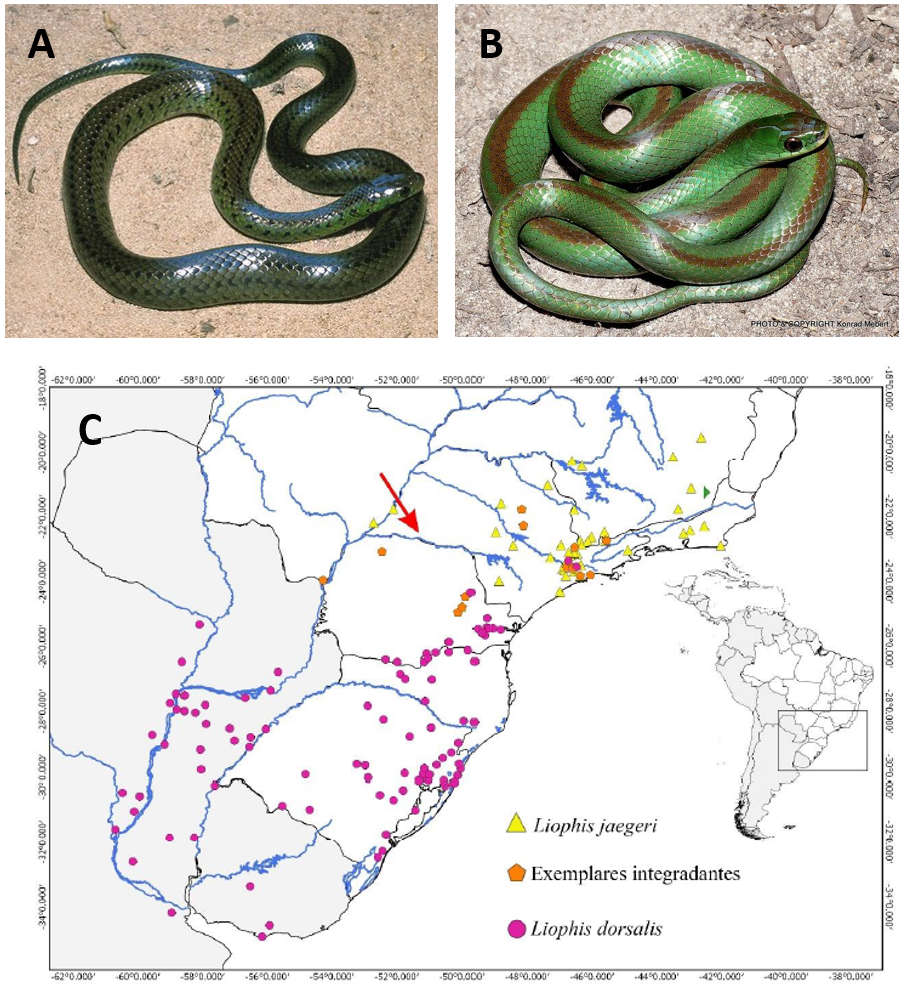
\includegraphics{../Projeto curso R/Figs/Imagem1.png} \textbf{Figura 1}:
A: \emph{Liophis jaegeri}, Foto: Ricardo Sawaia; B: \emph{Liophis
dorsalis}, Foto: Konrad Mebert; C: Mapa de distribuição de \emph{Liophis
jaegeri} e \emph{Liohis dorsalis}, retirado de Souto (2016).

\hypertarget{objetivos}{%
\subsection{Objetivos}\label{objetivos}}

Analisar as variações do número de escamas ventrais e subcaudais, além
do comprimento rostro cloacal (CRC) e comprimento caudal (CC) das
espécies \emph{Liophis jaegeri} e \emph{Liophis dorsalis}.

\hypertarget{material-e-muxe9todos}{%
\subsection{Material e métodos}\label{material-e-muxe9todos}}

Foram examinados 116 exemplares identificados como Liophis jaegeri
provenientes das \textbf{seguintes coleções:}

\hypertarget{nacionais}{%
\paragraph{Nacionais:}\label{nacionais}}

\begin{itemize}
\item
  Coleção herpetológica do Museu Nacional/UFRJ, Rio de Janeiro, RJ
  (MNRJ);
\item
  Coleção herpetológica do Instituto Butantan, São Paulo, SP (IBSP);
\item
  Coleção de herpetologia do Museu de Zoologia da Universidade de São
  Paulo, São Paulo, SP (MZUSP);
\item
  Coleção de herpetologia do Museu de História Natural Capão da Imbuia,
  Curitiba, PR (MHNCI);
\item
  Coleção de herpetologia do Museu de Ciência e Tecnologia da PUC-RS,
  Porto Alegre, RS (MCP);
\item
  Coleção de herpetologia da Fundação Zoobotânica, Porto Alegre, RS
  (MCN).
\end{itemize}

\hypertarget{estrangeiras}{%
\paragraph{Estrangeiras:}\label{estrangeiras}}

\begin{itemize}
\item
  Coleção de herpetologia do Museo Argentino de Ciencias Naturales
  Bernardino Rivadavia, Buenos Aires, ARG (MACN);
\item
  Coleção de herpetologia da Universidad Nacional del Litoral, Santa Fé,
  ARG (UNL);
\item
  Coleção de herpetologia da Universidad Nacional del Nordeste,
  Corrientes, ARG (UNNEC);
\item
  Coleção de herpetologia da Fundación Miguel Lillo, Tucumán, ARG (FML).
\end{itemize}

\hypertarget{anuxe1lises-morfoluxf3gicas}{%
\subsubsection{Análises
morfológicas}\label{anuxe1lises-morfoluxf3gicas}}

As medições de CRC e CC foram realizadas por meio de fita métrica com
precisão de 1 cm. O sexo dos indivíduos foi determinado através de uma
incisão longitudinal na base da cauda para verificar a presença ou não
de hemipênis. Além disso, foram contabilizadas o número de escamas
ventrais e subcaudais.

Por meio do programa RSudio (Versão 1.2.5003) foram realizadas análises
exploratórias dos dados e posterioremente foram gerados gráficos com o
intuito de visualizar as diferenças no número de escamas ventrais,
subcaudais, comprimento rostro cloacal (CRC) e comprimento caudal (CC)
entre as espécies.

\hypertarget{resultados-e-discussuxe3o}{%
\subsection{Resultados e discussão}\label{resultados-e-discussuxe3o}}

\hypertarget{histogramas}{%
\paragraph{Histogramas}\label{histogramas}}

Histogramas foram gerados através dos códigos:

\begin{verbatim}
# Frequência do número de Escamas ventrais por espécie:

par(mfrow = c(1,2))
hist(Liophis_dorsalis$Esc_ventrais, las = 1)
hist(Liophis_jaegeri$Esc_ventrais, las = 1)
\end{verbatim}

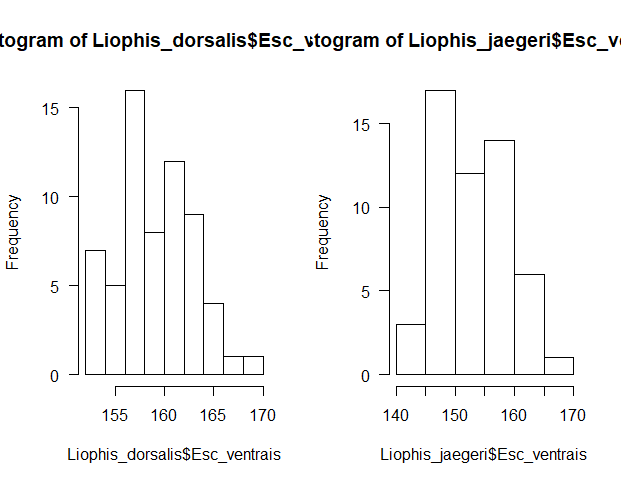
\includegraphics{../Projeto curso R/Figs/Freq_Ventrais_Especie.png}

\begin{verbatim}
# Frequência do número de Escamas subcaudais por espécie:

par(mfrow = c(1,2))
hist(Liophis_dorsalis$Esc_subcaudais, las = 1)
hist(Liophis_jaegeri$Esc_subcaudais, las = 1)
\end{verbatim}

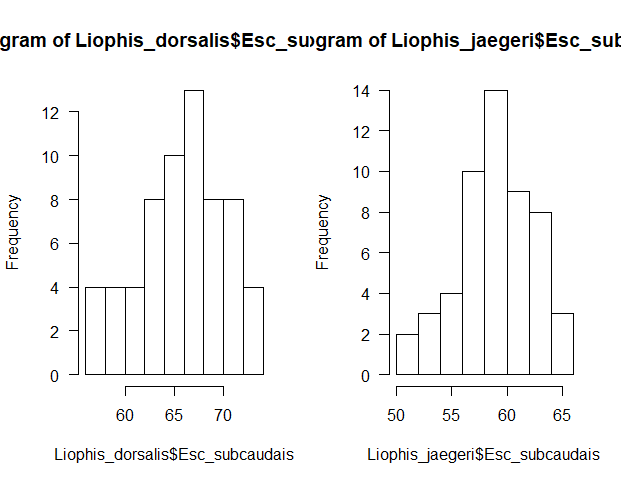
\includegraphics{../Projeto curso R/Figs/Freq_Subcaudais_Especie.png}

\begin{verbatim}
# Frequência de CRC por espécie:

par(mfrow = c(1,2))
hist(Liophis_dorsalis$CRC, las = 1)
hist(Liophis_jaegeri$CRC, las = 1)
\end{verbatim}

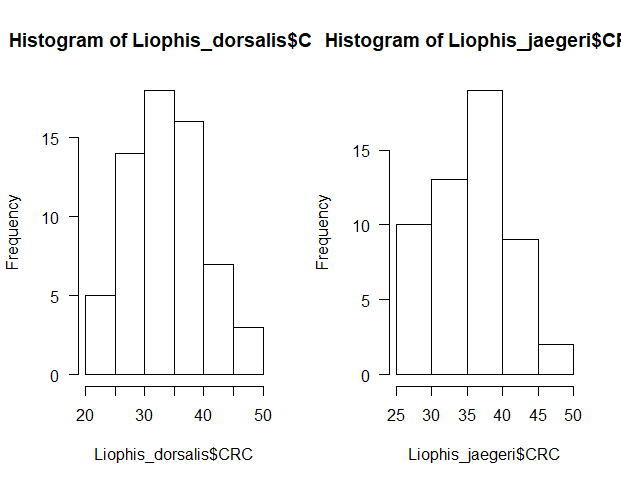
\includegraphics{../Projeto curso R/Figs/Freq_CRC_Especie.png}

\begin{verbatim}
# Frequência de CC por espécie:

par(mfrow = c(1, 2))
hist(Liophis_dorsalis$CC, las = 1)
hist(Liophis_jaegeri$CC, las = 1)
\end{verbatim}

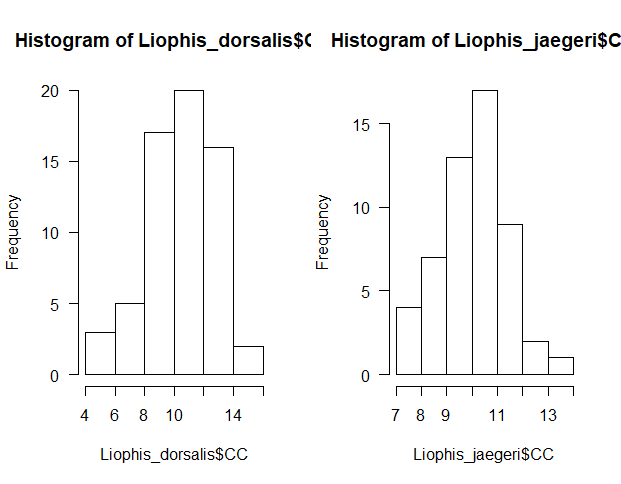
\includegraphics{../Projeto curso R/Figs/Freq_CC_Especie.png}

\hypertarget{boxplot}{%
\paragraph{Boxplot}\label{boxplot}}

Os gráficos de boxplot foram gerados através dos códigos:

\begin{verbatim}
# Boxplot das escamas ventrais e subcaudais por espécie:

par(mfrow = c(1,2))
boxplot(Esc_ventrais ~ Especie, data = Dados, las = 1)
boxplot(Esc_subcaudais ~ Especie, data = Dados, las = 1)
\end{verbatim}

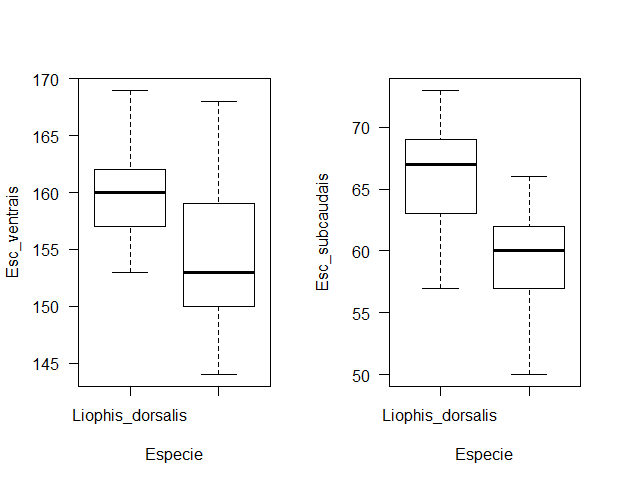
\includegraphics{../Projeto curso R/Figs/Rplot_Esc_Especies.png}

\begin{verbatim}
# Boxplot das escamas ventrais e subcaudais por sexo

par(mfrow = c(1,2))
boxplot(Esc_ventrais ~ Sexo, data = Dados, las = 1)
boxplot(Esc_subcaudais ~ Sexo, data = Dados, las = 1)
\end{verbatim}

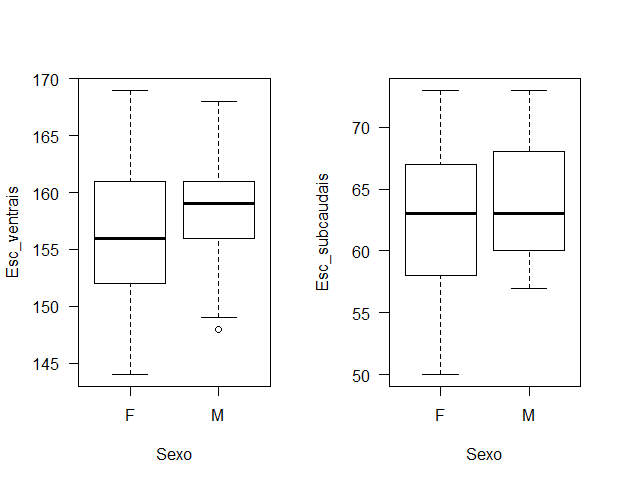
\includegraphics{../Projeto curso R/Figs/Rplot_Esc_sexo.png}

\begin{verbatim}
# Boxplot do comprimento CRC e CC por espécie

par(mfrow = c(1,2))
boxplot(CRC ~ Especie, data = Dados, las = 1)
boxplot(CC ~ Especie, data = Dados, las = 1)
\end{verbatim}

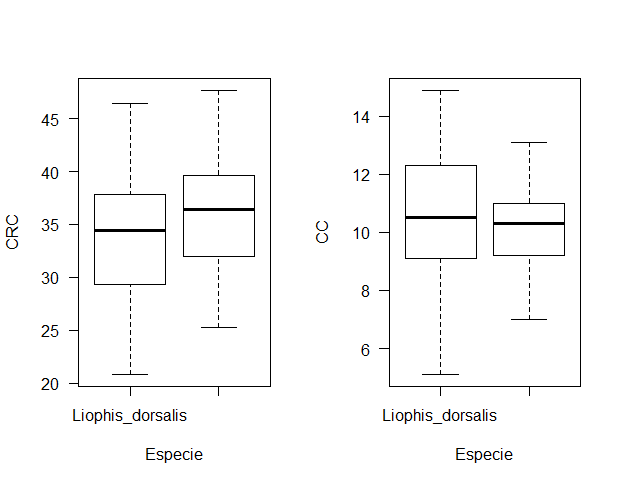
\includegraphics{../Projeto curso R/Figs/Rplot_CRC_CC_Especie.png}

\begin{verbatim}
# Boxplot do comprimento CRC e CC por sexo

par(mfrow = c(1,2))
boxplot(CRC ~ Sexo, data = Dados, las = 1)
boxplot(CC ~ Sexo, data = Dados, las = 1)
\end{verbatim}

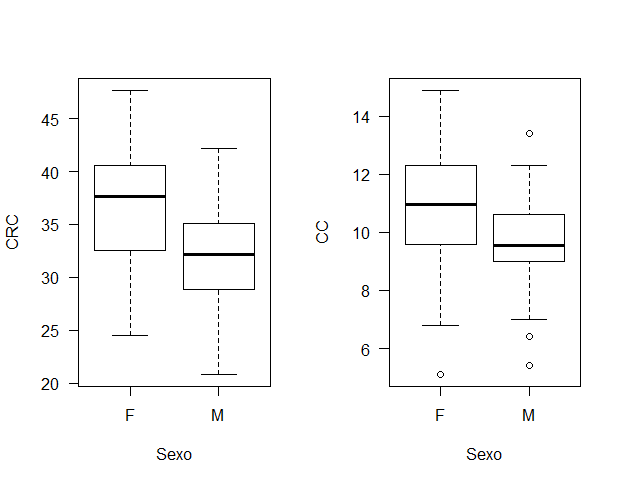
\includegraphics{../Projeto curso R/Figs/Rplot_CRC_CC_Sexo.png}

\end{document}
